\chapter{Testing}\label{chapter:testing}
\section{Infrastructure}
The infrastructure for the project is divided in two parts:
\begin{itemize}
	\item the Nix \cite{nix} ``glue'',		
	\item some python utilities to call and confront provers.
\end{itemize}
In nix everything must be packaged as something called a derivation: a declarative recipe specifying all the needed programs (as other derivations) and the steps necessary to build the source.
These steps are executed in a environment containing only the specified programs and little else.

Derivations are written for all the programs we interact with:
\begin{itemize}
	\item the provers, such as APLL or llprover;
	\item the formula generator adapted from APLL described in Section \ref{sec:formula generator};
	\item the LLTP parser.
\end{itemize}
All these, together with one for the python environment, are then used to define a single development environment to run the Jupyter notebook with all the necessary dependencies.
Furthermore, having used ``flakes'' (a nix experimental feature), all dependencies are locked to a certain commit thus ensuring better reproducibility.

The main logic for the benchmarking and testing is defined in the python module \texttt{testprover.py}.
Here for simplicity we assume that the executable of a prover returns a code of 0 if it has found a proof, or any other number otherwise.
This condition is already met by our prover and by llprover; for APLL we instead provide a wrapper.

Defining the call to our prover using this library is as simple as writing
\begin{minted}[linenos]{python}
pc = Registered()

@pc.register('sat-ll')
@call_prover(PrefixTree.SAT_LL_DICT)
def call_sat_prover(premises, conclusions):
  return [ 'sat-ll'
    , '-b', '3'
    , f'{premises} |- {conclusions}'
    ]
\end{minted}
The function defining a call to a prover must take as inputs two arguments, the list of premises and the list of conclusions (using the format described in Section \ref{sec:prefix}), and return the command calling the prover as a list.
The innermost decorator (line 3) then accepts a dictionary, and returns a function which automatically calls the prover above with a test entry (as in Section \ref{sec:file format}), times it, and eventually terminates the process if it takes too much.
Lastly, the outermost decorator (line 4) simply adds an entry \texttt{'sat-ll'} associated with the prover call to the register \texttt{pc}.
This register is just an association name to function, and it is what is actually passed to the benchmarking functions which will use the names in the output tables.

The library then provides two functions:
\begin{itemize}
	\item \texttt{testall} accepts a single prover and a test suite; the function checks if the output of the prover corresponds to the expected value for the test;
	\item \texttt{benchmark} accepts a register and a test suite and returns the times and outcomes of each prover.
		This function is used to compare different provers.
\end{itemize}
All the outputs of the functions above are pandas \texttt{DataFrame}s, which means that they can be easily queried, dumped to CSV, aggregated, or visualized using most plotting libraries.
For example let \texttt{out} be the output of a call to \texttt{testall} with some prover and test suite:
\begin{minted}{python}
out['outcome'].map(lambda x: x == Outcome.SUCCESS).all()
len(out[(out['outcome'] == Outcome.FAILURE) 
       | (out['outcome'] == Outcome.TIMEOUT)])
\end{minted}
test respectively whether all the tests succeeded and the number of failed tests.

\subsection{Prefix format}\label{sec:prefix}
Since for benchmarking we may interface with many different provers -- each with its own syntax for expressions -- the need arose for a common format which was easy to parse and translate.
For this purpose we define a prefix format for linear logic formulae inspired by the format used by \cite{TarauPaiva} for implicational formulae:
\begin{table}[H]
	\centering
	\begin{tabular}{cc}
		\hline
			formula & symbol \\
		\hline
		\hline
			$\phi_A \llten \phi_B$  & \texttt{*AB} \\
			$\phi_A \llpar \phi_B$  & \texttt{|AB} \\
			$\phi_A \llplus \phi_B$ & \texttt{+AB} \\
			$\phi_A \llwith \phi_B$ & \texttt{\&AB} \\
			$\phi_A \lolli \phi_B$  & \texttt{@AB} \\
			$\llnot{\phi_A}$        & \texttt{\^{}A} \\
			$\llwn{\phi_A}$         & \texttt{?A} \\
			$\llbang{\phi_A}$       & \texttt{!A} \\
	\end{tabular}
\end{table}
Each single character not representing an operator is considered as a variable name.
Longer names can be specified by enclosing them in single quotes as in \texttt{'varname'}.
As an example we give the translation of DeMorgan for the tensor:
$$ \mathrm{prefix}(\llnot{(a \llten b)} \lolli \llnot{a} \llpar \llnot{b}) = \text{\texttt{@\^{}ab|\^{}a\^{}b}} $$

% Since most one of the datasets we use is LLTP % cite
% , which is written in TPTP's format % cite
% , we define a parser for this using Haskell's parser generator happy. % cite

\subsection{File formats}\label{sec:file format}
We use json as a standard format to store the tests, because of its vast adoption by most programming languages.
A test suite is thus defined as a list of test cases; where a test case is just an object with these three mandatory fields:
\begin{center}
\begin{tabular}{l l}
	\textbf{id} &  		\parbox{11cm}{is a number with the sole purpose of tracing back the test case from the output;} \\
	\textbf{premises} & 	\parbox{11cm}{is a list of premises as prefix formulae;} \\
	\textbf{conclusions} & 	\parbox{11cm}{is a list of conclusions as prefix formulae.} \\
\end{tabular}
\end{center}
For example
\begin{minted}{json}
{
	"id": 1,
	"premises": [ "^*ab" ],
	"conclusions": [ "|^a^b" ]
}
\end{minted}
is the test case representing $\llnot{(a \llten b)} \vdash \llnot{a} \llpar \llnot{b}$.
Other arbitrary fields may be present; for example we will use the following optional fields:
\begin{center}
	\begin{tabular}{ l l }
		\textbf{thm} & 		\parbox{11cm}{tells whether this test case is a tautology or not, may be null;} \\
		\textbf{*, +, ?, ...} & \parbox{11cm}{is the number of times a specific connective appears in the test case;} \\
		\textbf{notes} & 	\parbox{11cm}{is a human readable string about the test case, e.g. its infix representation;} \\
		\textbf{size} & 	\parbox{11cm}{is an indicative number of the size of the formula;} \\
		\textbf{atoms} & 	\parbox{11cm}{is the upper bound on the number of atoms.}
	\end{tabular}
\end{center}
The fields \texttt{size} and \texttt{atoms} will be further explained in Section \ref{sec:formula generator}.

\subsection{Formula generation}\label{sec:formula generator}
One of the sources of formulae we'll use in Section \ref{sec:benchmarking} is APLL's random formula generator.
The version we'll use is a slight modification of it, where:
\begin{itemize}
	\item the output is in the json format described in Section \ref{sec:file format};
	\item one can choose whether to generate normalized formulae or not;
	\item one can choose which connectives appear in the generated formula.
\end{itemize}
% TODO: sistemo
A noteworthy detail is how the parameters \texttt{size} and \texttt{atoms} mentioned in Section \ref{sec:file format} are defined, as these are directly related to how the formulae are generated:
\begin{itemize}
	\item when one specifies a number of atoms, the generator initializes an array containing that number of atoms, their negations, and the constants $\bot, \top, \dots$.
		During the generation of the formula this array is randomly accessed, choosing an element when needed.
		This means that \texttt{atoms} represents an upper bound to the number of different atoms that may appear in the formula, not their exact number.
	\item when a formula is generated, at each step it is chosen whether to generate a unary or binary connective based on a threshold:
		\begin{itemize}
			\item if a unary connective is chosen, the process continues with a size of 
				$$\text{\texttt{size}} - 1$$
			\item if a binary connective is chosen, the program chooses a random value between 0 and \texttt{size}, and it generates the two branches of the formula, with size respectively $k$ and $\text{\texttt{size}} - k$.
		\end{itemize}
		This means that \texttt{size} is just an indicative value of the number of connectives in the formula.
\end{itemize}

\section{Benchmarking}\label{sec:benchmarking}
% Finding a comprehensive test suite for linear logic, moreover one which is not made up mostly of translations of other theorems to linear logic, is not easy.
% Most of the theorems we use for testing are llprover's %cite
We'll mainly use three sources for formulae: llprover's tests; LLTP \cite{LLTP}, especially the translations of Kleene's intuitionistic formulae; and randomly generated formulae made by the generator described in \ref{sec:formula generator}.
Out of these, llprover's tests are composed primarily of simple linear logic tautologies, such as the DeMorgan rules; for this reason these tests are just used to quickly check for obvious bugs.

% TODO: sistemo
Randomly generated formulae will be used only for non-exponential test for the following reasons:
\begin{itemize}
	\item datasets of linear logic theorems without exponentials are rare and most often the formulae in them do not have a significant size; 
	\item when dealing with exponential formulae a prover may wrongfully deem a true formula false, just because it exhausted its bound.
		This problem is exacerbated when dealing with generated tests: since the expected output is not known we do not know if the prover terminated because of the bound, or if the test is actually a non-theorem.
\end{itemize}

Using random formulae we can see that our prover outperforms APLL (and llprover) when dealing with formulae rich in multiplicatives (Figure \ref{fig:mll bars} and Table \ref{table:mll}).
\begin{figure}[H]
	\centering
	\begin{subfigure}{0.49\textwidth}
		\centering
		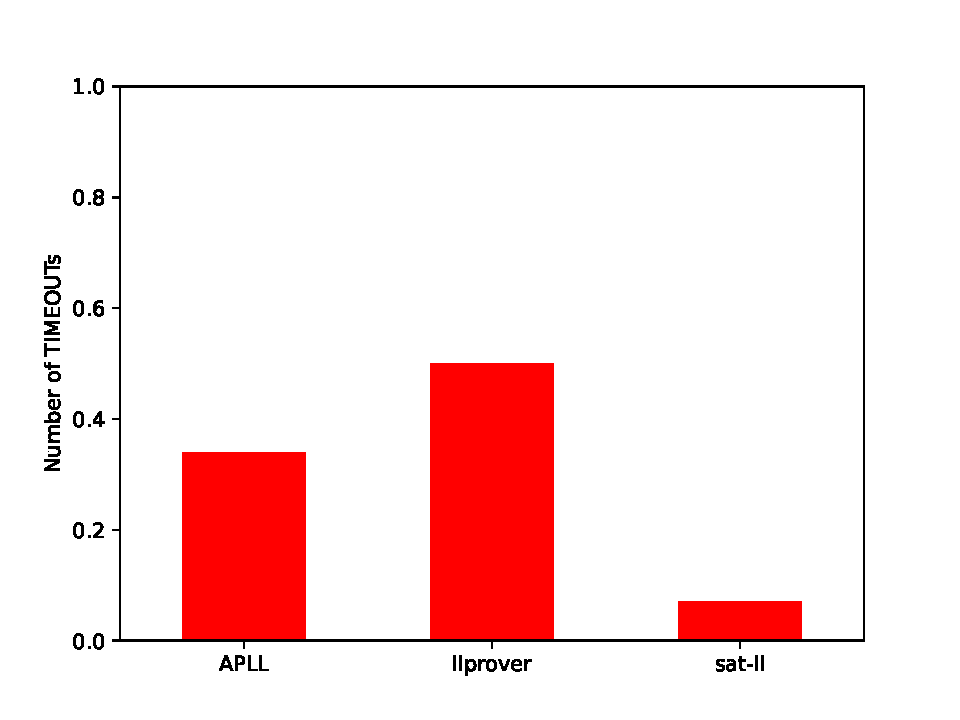
\includegraphics[scale=0.5]{figures/mll.pdf}
		\caption{Multiplicative case}
		\label{fig:mll bars}
	\end{subfigure}
	\begin{subfigure}{0.49\textwidth}
		\centering
		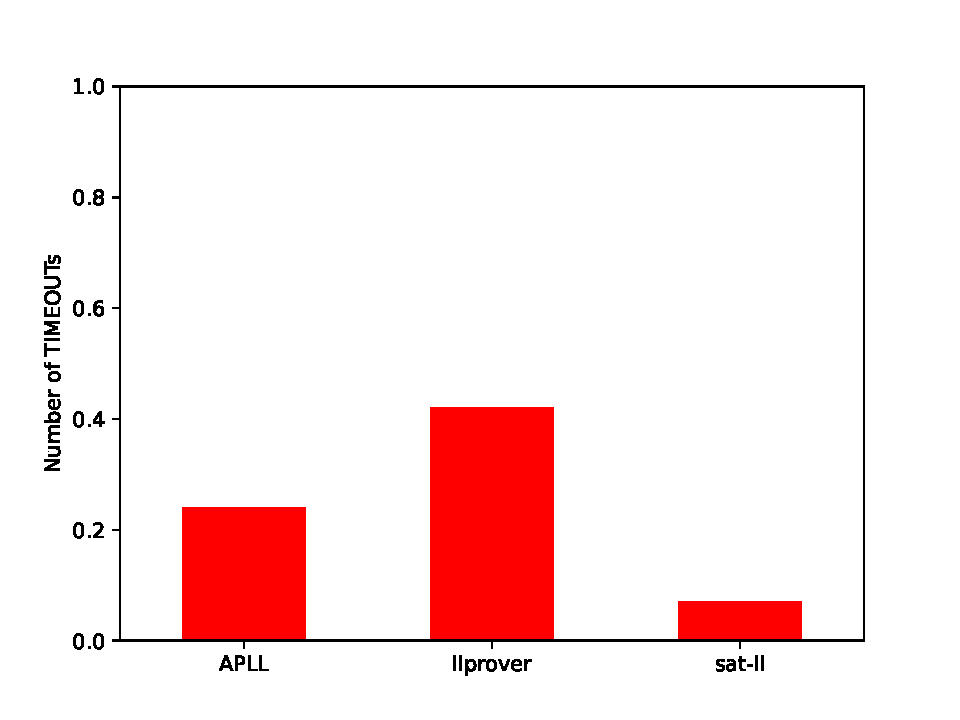
\includegraphics[scale=0.5]{figures/mall.pdf}
		\caption{Multiplicative and additive case}
		\label{fig:mall bars}
	\end{subfigure}
	\caption{Percentage of number of timeouts out of a hundred formulae}
\end{figure}
\begin{table}[h!]
	\begin{subtable}{\textwidth}
		\centering
		{\footnotesize
		\begin{tabular}{| l c c c c | }
			\hline
			\textbf{prover} & \textbf{timeouts} & \textbf{successes} & \textbf{success rate} & \textbf{avg. time (succ.)} \\
			\hline
			\hline
			APLL & 34 & 66 & $0.66$ & \qty{1.441}{\second}  \\
			llprover & 50 & 50 & $0.50$ & \qty{3.006}{\second}  \\
			sat-ll & 7 & 93 & $0.93$ & \qty{1.874}{\second} \\
			\hline
		\end{tabular}
		}
		\caption{Data corresponding to Figure \ref{fig:mll bars}}
		\label{table:mll}
	\end{subtable}\vspace{.5cm}
	\begin{subtable}{\textwidth}
		\centering
		{\footnotesize
		\begin{tabular}{| l c c c c | }
			\hline
			\textbf{prover} & \textbf{timeouts} & \textbf{successes} & \textbf{success rate} & \textbf{avg. time (succ.)} \\
			\hline
			\hline
			APLL & 24 & 76 & $0.76 $ & \qty{1.213}{\second}  \\
			llprover & 42 & 58 & $0.58$ & \qty{0.807}{\second}  \\
			sat-ll & 7 & 93 & $0.93$ & \qty{1.289}{\second} \\
			\hline
		\end{tabular}
		}
		\caption{Data corresponding to Figure \ref{fig:mall bars}}
		\label{table:mall}
	\end{subtable}
	\caption{Non exponential tests.}
\end{table}
We can also see that in the multiplicative and additive case the difference begin to level (Figure \ref{fig:mall bars} and Table \ref{table:mall}).
The additive case is not that significant as the formulae remain manageable and no major differences can be seen.
When reviewing these outputs it is important to remember that randomly generated tests lack the structure of real formulae, and this may impact the quality of the measurement.
All these test were done generating suites of 100 tests using a timeout of \qty{60}{\second}:
\begin{itemize}
	\item Figure \ref{fig:mll bars}'s tests were composed of formulae of \texttt{size} 100, and \texttt{atoms} 50, using just tensor ($\displayten$) and par ($\displaypar$) as connectives;
	\item Figure \ref{fig:mall bars}'s tests were composed of formulae of \texttt{size} 500, and \texttt{atoms} 250, with all the connectives, except the exponentials ($\displayten, \displaypar, \displaywith$ and $\displayplus$)
\end{itemize}

\begin{table}[h!]
	\begin{subtable}{\textwidth}
		\centering
		{\footnotesize
		\begin{tabular}{ | l c c c c c c | }
			\hline
			\textbf{prover} & \textbf{timeouts} & \textbf{failures} & \textbf{successes} & \textbf{success rate} & \textbf{avg. (succ.)} & \textbf{avg. (tot.)} \\
			\hline
			\hline
			APLL & 0 & 17 & 71 & $\approx 0.80$ & \qty{0.035}{\second} & \qty{0.326}{\second} \\
			llprover & 20 & 6 & 62 & $\approx 0.70$ & \qty{0.981}{\second} & \qty{2.179}{\second} \\
			sat-ll & 5 & 15 & 68 & $\approx 0.77$ & \qty{0.443}{\second} & \qty{0.496}{\second} \\
			\hline
		\end{tabular}
		}
		\caption{Outputs for KLE-cbv}
		\label{table:KLE-cbv}
	\end{subtable}\vspace{.5cm}
	\begin{subtable}{\textwidth}
		\centering
		{\footnotesize
		\begin{tabular}{ | l c c c c c c | }
			\hline
			\textbf{prover} & \textbf{timeouts} & \textbf{failures} & \textbf{successes} & \textbf{success rate} & \textbf{avg. (succ.)} & \textbf{avg. (tot.)} \\
			\hline
			\hline
			APLL & 0 & 16 & 72 & $\approx 0.80$ & \qty{0.037}{\second} & \qty{0.055}{\second} \\
			llprover & 20 & 6 & 62 & $\approx 0.70$ & \qty{1.709}{\second} & \qty{3.253}{\second} \\
			sat-ll & 4 & 18 & 66 & $\approx 0.75$ & \qty{0.130}{\second} & \qty{0.185}{\second} \\
			\hline
		\end{tabular}
		}
		\caption{Outputs for KLE-cbn}
		\label{table:KLE-cbn}
	\end{subtable}
	\caption{Exponential tests.}
\end{table}
We now show the results of running the provers on two datasets: KLE-cbn and KLE-cbv, respectively the call-by-name and call-by-value translations of Kleene's theorems.
These translations introduce a high number of exponentials; this causes -- as said before -- some failures not due to bugs, but because of the the exhausted number of contractions.
The benchmarks are done using a timeout of \qty{60}{\second} and a bound of 3.
It can be seen in Table \ref{table:KLE-cbv} and \ref{table:KLE-cbn} that the differences of the previous tests are completely leveled, and instead our prover performs slightly worse than APLL.

Overall, since llprover uses incremental search, its times are often skewed towards the slower side.
Similarly our prover is consistently slightly slower that APLL, this difference is negligible and can be probably ascribed to differences languages' runtimes.

